\section{Introduction}
The standard model of particle physics
(SM) is one of the most precise theories to this date.
Although the SM describes the interaction of the fundamental particles
with enormous precision, it is known to have its limitations.
For example it can not explain the matter-antimatter asymmetry in the universe,
nor does it include a description of interactions at the Planck-scale.
Extensions of the SM including new interactions and particles are called
\enquote{new physics} (NP).
In the SM the three leptons
$e, \mu, \tau$ only differ by their mass.
In all other properties they are interchangeable,
because they transform the same under the $\symup{SU(3)\times SU(2)\times U(1)}$
gauge group of the SM.
This Lepton Flavor Universality (LFU) can be viewed
as a key prediction of the SM.

Recent measurements of the LHCb experiment hint at deviations from LFU, which would be a clear sign of NP effects.
There are theoretical models to explain LFU in beyond standard model processes, such as lepto-quarks (LQ) which
directly couple leptons to quarks.

\subsection{$B^+\to K^+l^{+} l^{-}$ decays}
In the SM some decay rates can be predicted with high accuracy
The $B^+\to K^+l^{+} l^{-}$ and similar decays happen with $b\to s l^+l^-$
quark transitions. They contain a hadron in the final state and
are forbidden at tree level.
The lowest order diagram contributing in the SM is a
penguin diagram as seen in \autoref{fig:SMbkll}.
For that reason the branching fraction of that process
is suppressed on the order of
$\mathcal{O}(10^{-6})$ \cite{Zyla:2020zbs}.
This is good to observe NP effects,
since there are NP models, where this decay can happen
on tree-level.
An example of such a NP process is the
lepto-quark mediated diagram in \autoref{fig:BSMbkll}.

Similar processes with $b\to sl^+ l^-$ transitions,
allow similar analysis.
They provide different observables than
similar measurements without a meson in the final state.
\begin{figure}
	\centering
	\begin{tikzpicture}
		\begin{feynman}
			\vertex (b1) {$\overline b$};
			\vertex [right=of b1] (b2);
			\vertex [right=of b2] (b3);
			\vertex [right=of b3] (b4) {$\overline s$};

			\vertex [above=.8 of b1] (u1) {$u$};
			\vertex [above=.8 of b4] (u2) {$u$};

			\vertex at ($(b2)!0.5!(b3)!1!-90:(b3)$) (g1);
			\vertex [below=1.5 of b3] (g2);
			\vertex [below=1.2 of b4] (l1) {\(\ell^{+}\)};
			\vertex [below=.6 of l1] (l2) {\(\ell^{-}\)};

			\diagram* {
			(u1) -- [fermion] (u2),
			(b1) -- [anti fermion] (b2) -- [boson, edge label={$W^+$}] (b3) -- [anti fermion] (b4),
			(b2) -- [anti fermion, bend right] (g1) -- [anti fermion, bend right] (b3),
			(g1) -- [photon, bend right, edge label'={$\gamma/Z^0$}] (g2),
			(l1) -- [fermion, bend right] (g2) -- [fermion, bend right] (l2),
			};

		\end{feynman}
		\draw[decorate, decoration={brace, amplitude=5pt},line width=1pt](b1.south west) --node[left] {$B^+ \ $} (u1.north west);
		\draw[decorate, decoration={brace, amplitude=5pt},line width=1pt](u2.north east) --node[right] {$\ K^+ \ $} (b4.south east);
		\node [above=0.15 of g1]  {$\overline u, \overline c, \overline t$};
	\end{tikzpicture}
	\caption{\label{fig:SMbkll} SM lowest order diagram of the $B^+\to~K^+l^{+}~l^{-}$ decay.}%
\end{figure}

\begin{figure}
	\centering
	\begin{tikzpicture}
		\begin{feynman}
			\vertex (b1) {$\overline b$};
			\vertex [right=of b1] (b2);
			\vertex [right=of b2] (b3);
			\vertex [right=of b3] (b4) {$\overline s$};

			\vertex [above=.8 of b1] (u1) {$u$};
			\vertex [above=.8 of b4] (u2) {$u$};

			\vertex [below=1.2 of b4] (l1) {\(\ell^{+}\)};
			\vertex [below=.7 of l1] (l2) {\(\ell^{-}\)};

			\diagram* {
			(u1) -- [fermion] (u2),
			(b1) -- [anti fermion] (b2) -- [scalar, edge label={$LQ$}] (b3) -- [anti fermion] (b4),
			(l1) -- [fermion, bend left] (b3),
			(l2) -- [fermion, bend left] (b2),
			};

		\end{feynman}
		\draw[decorate, decoration={brace, amplitude=5pt},line width=1pt](b1.south west) --node[left] {$B^+ \ $} (u1.north west);
		\draw[decorate, decoration={brace, amplitude=5pt},line width=1pt](u2.north east) --node[right] {$\ K^+ \ $} (b4.south east);
	\end{tikzpicture}
	\caption{\label{fig:BSMbkll} NP example of the $B^+\to~K^+l^{+}~l^{-}$ decay with lepto-quark interaction.}%
\end{figure}





\section{Lepton Flavor Universality Tests}
In the last decade multiple tensions with SM predictions were observed in $b\to s l^+l^-$ transitions.
The deviation in observables from SM predictions, are called \enquote{flavor anomalies}.
These deviations recently reached the $\num{3}\sigma$ level, based on proton-proton collision data
at the LHCb detector.
Since the calculations in quantum chromo dynamics (QCD) rely on lattice-qcd predictions, because
of the non-pertubative nature of QCD,
the resulting uncertainties in QCD effects are high.
Since changing leptons does not affect QCD calculations because of LFU,
it is possible to define observables, which are independent from QCD uncertanties,
since they cancel. One class of theoretically clean observables is \cite{Hiller2004}
\begin{equation}
	R_{H}:= \frac{\int^{q_{\mathrm{max}}^2}_{q_{\mathrm{max}}^2}\frac{\dif \mathcal{B}(B\to H\mu^+\mu^-)}{\dif q^2} \dif q^2}{
		\int^{q_{\mathrm{max}}^2}_{q_{\mathrm{max}}^2}\frac{\dif \mathcal{B}(B\to He^+e^-)}{\dif q^2} \dif q^2
	} \overset{\mathrm{SM}}{\approx} 1.
\end{equation}
$\mathcal{B}$ is the branching ratio of the given process, where $H$ can be a hadron ($H=K$ in our case)
or even a collection of particles. The differential branching fractions are
integrated over the invariant mass squared of the two leptons
in the \emph{same} region $q^2~\in~(q_{\mathrm{min}}^2,~q_{\mathrm{max}}^2)$.
These observables are free from QCD uncertanties.
For example in the SM without radiative (QED) corrections
$R_{K}=\num{1.00030}_{-\num{0.00007}}^{+\num{0.00010}}$
for $q^2\in(1, 6)\si{\giga\electronvolt}$
has a relative uncertainty in the order of
$\mathcal{O}(10^{-4})$\cite{Hiller}.
Adding QED corrections (which are relevant only because
of the different electron and muon mass)
The full uncertainty of $R_K$ is in the order
of $\mathcal{O}(\SI{1}{\percent})$ \cite{Bordone2016}.
This means that a big deviation from unity in this value
is a big indication for NP.
Until this year only a part of Run 2
LHCb data was analised corresponding (together with Run 1 data) to
\SI{5}{\femto\barn\tothe{-1}} of data.
Shown in \autoref{fig:RKearlier} and \autoref{fig:RKstarearlier}
part of the LHCb dataset already showed a small
deviation from unity at the $2\sigma$ level.
At LHCb $q^2$ is always chosen to be smaller than
\SI{6}{\giga\electronvolt}, to reduce contributions
from the $J/\Psi$ resonance.
\begin{figure}
	\centering
	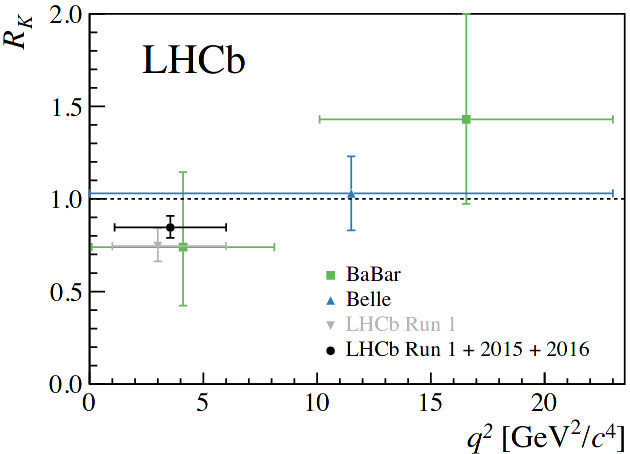
\includegraphics[width=0.6\linewidth]{media/RK.png}
	\caption{Measurements of $R_K$ \cite{petridis2021test}. The LHCb measurement with Run 1 and 2015/16 data corresponds to \SI{5}{\femto\barn\tothe{-1}}.
		It hints at SM tension at the $2\sigma$ level.}%
	\label{fig:RKearlier}
\end{figure}
\begin{figure}
	\centering
	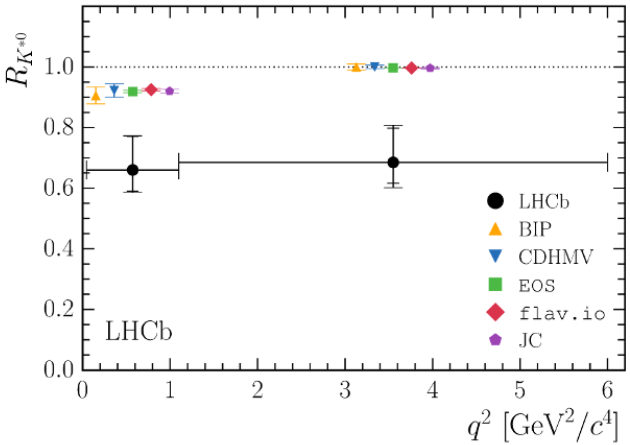
\includegraphics[width=0.6\linewidth]{media/RKstar.png}
	\caption{Measurements of $R_{K^{*0}}$ \cite{petridis2021test}. The LHCb measurement corresponds to  \SI{3}{\femto\barn\tothe{-1}}.
		It hints at SM tension around the $2\sigma$ level.}%
	\label{fig:RKstarearlier}
\end{figure}

\section{$\bfiftextbf{R_K}$ with the full LHC\lowercase{b} dataset}
This year the remaining Run 2 LHCb data recorded in 2017 and 2018
was added to the earlier \SI{5}{\femto\barn\tothe{-1}}.
This adds \SI{4}{\femto\barn\tothe{-1}} to the dataset
roughly doubling the amount of observed decays.

The same analysis strategy as in the smaller dataset is used and the
results are double checked.

It was already established in the earlier section that $R_K$ provides
a theoretically clean prediction.
The experimental measurement of $R_K$ is challenging because
of the different behavior of electrons and muons in the detector.
The muons pass the detector nearly unaffected and are stopped in the end
by the muon stations.
Electrons on the other hand radiate bremsstrahlung and for that
reason their energy reconstruction is more difficult
and the mass resolution is poorer.
Most electrons emit a energetic bremsstrahlungs photon before the magnet and
are then curved and emit more photons downstream. The photons are detected by the
electromagnetic calorimeter (ECAL).
This situation is illustrated
in \autoref{fig:bremsstrahlung}.
The lost energy can be added back by choosing
the clusters directed towards the electron direction before the magnet ($E_{T}>\SI{75}{\mega\electronvolt}$).
Even after this recovery the electron mass distribution is still not as sharp as the muon one, which can
be seen in \autoref{fig:masses}.
More differences stem from differences in the triggers, particle identification and tracking efficiency.
Controlling the experimental differences is key to the analysis strategy.
\begin{figure}
	\centering
	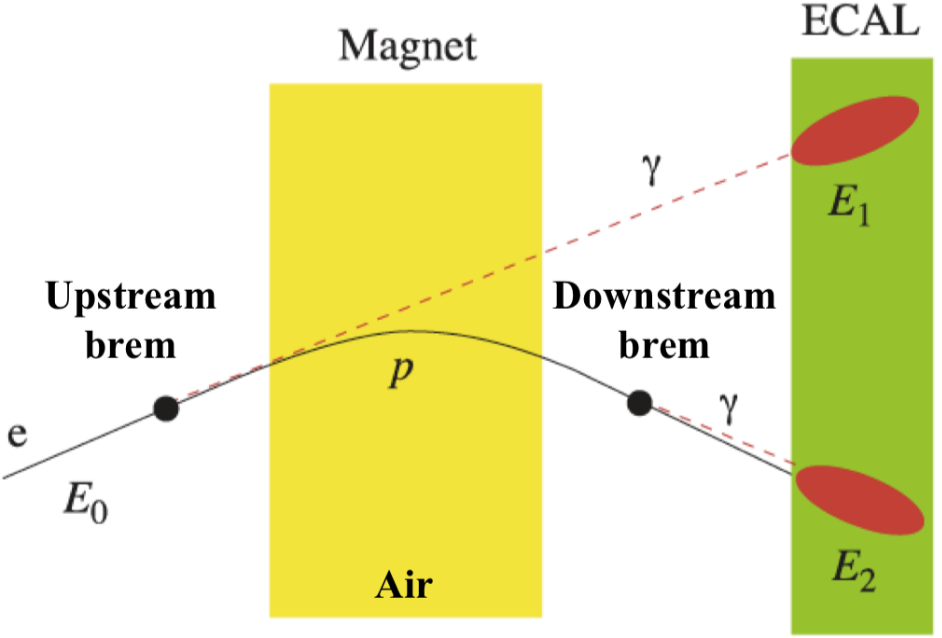
\includegraphics[width=0.8\linewidth]{media/electronbrems.png}
	\caption{Reconstruction of the electron energy at LHCb with bremsstrahlung \cite{petridis2021test}.}%
	\label{fig:bremsstrahlung}
\end{figure}

\begin{figure}[h]
	\centering
	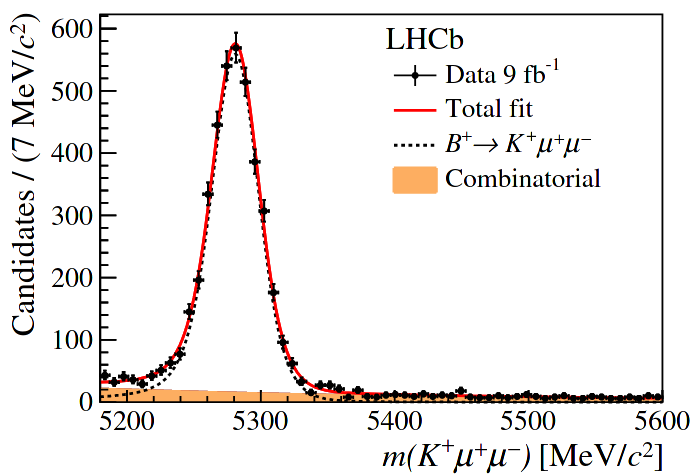
\includegraphics[width=0.8\linewidth]{media/Mmumu.png}
	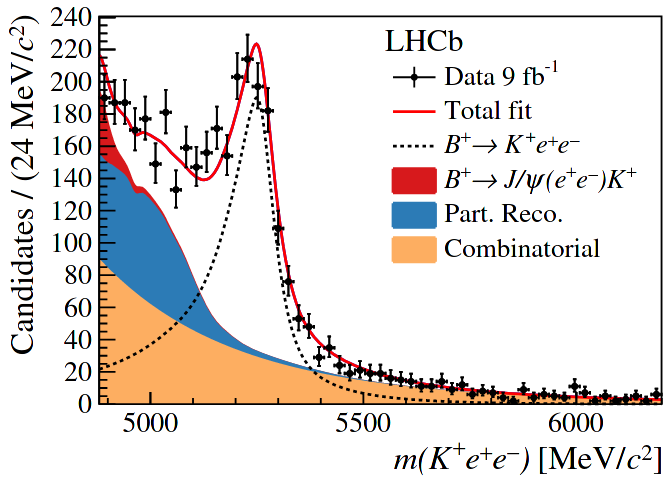
\includegraphics[width=0.8\linewidth]{media/Mee.png}
	\caption{Invariant mass distribution of the final state particles in the muon muon decay (top) and the electron electron decay (bottom) \cite{petridis2021test}.
		The energy resolution of the muon is notably better.}%
	\label{fig:masses}
\end{figure}

\subsection{The double ratio strategy}
To suppress the systematic effects coming from electron/muon differences 
the branching ratios can be measured relative to a well understood control channel. 
The channel of choice is the $B^+\to K^+j/\psi(\ell^+\ell^-)$ due to its high similarity 
with the channel of interest. They share identical selections except the cut on $q^2$.
Furthermore the $J/\psi$ mode is known to obey LFU within $\mathcal{O}(10^{-4})$ \cite{Moise:2021nje}.
The experimental observable can than be defined as
\begin{align}
	\label{eqn:rkexp}
	R_K & = \l .\frac{\mathcal{B}(B\to K^+\mu^+\mu^-)}{\mathcal{B}(B\to K^+J/\psi(\mu^+\mu^-))} \r/
	\frac{\mathcal{B}(B\to K^+e^+e^-)}{\mathcal{B}(B\to K^+J/\psi(e^+e^-))} \nonumber               \\
	    & = \l . \frac{N_{\mu}}{\epsilon_\mu}\frac{\epsilon_{J/\psi(\mu)}}{N_{J/\psi(\mu)}} \r/
	\frac{N_{e}}{\epsilon_e}\frac{\epsilon_{J/\psi(e)}}{N_{J/\psi(e)}}.
\end{align}
Where $\epsilon$ are the efficiencies of the indicated decays and $N$ their yields.
To clearify the expression the integrals in the first line were omitted.

The invariant mass distribution of the final state particles is fitted to get the yields
and the efficiencies are calculated using simulated events. 
Some aspects are modeled imperfectly by the simulation, 
and for that reason the efficiencies need calibration, which 
is done with control channels in data. 


\subsection{Selection and backgrounds}
To remove unwanted backgrounds in the dataset 
further selections have to be applied.
Removing backgrounds decays with the same (detectable) 
final state can be done by applying mass vetoes. 
For example the decay $B^+\to~\anti D^0(\to~K^+e^-\nu)e^+\anti \nu$
has the same final state, since the neutrinos are undetectable.
To remove this the invariant mass is constrained to 
furfill the condition $m(K^+ e^-) > m(D^0)$.
Another type of background is misidentified background, where e.g. 
pions get identified as electrons. 
This can be removed by requiring a high value for the identification 
probability of the electron (electron PID).
Combinatorial background, where unrelated events are counted towards 
a signal event, 
can be removed via a multivariate selection which takes multiple 
variables at the same time into account. 
This is usually done via statistical learning techniques like 
a boosted decision tree (BDT).

Even more backgrounds can be suppressed by 
choosing a $m(K^+\ell^+\ell^-)$ window. 
This is shown  
in \autoref{fig:backgrounds}
where multiple simulated backgrounds can be seen. 
The dominant ones are the $J/\psi$ channel which leaked 
into the invariant mass region of interest and the
partially reconstructed decay $B\to K^+ \pi^-e^+e^-$, where the pion 
was not reconstructed. 

The simulation is calibrated through control data 
for trigger efficiency, PID efficiency, $B^+$ kinematics and 
the resolutions of $q^2$ and $m(K^+e^+e^-)$.

\begin{figure}
	\centering
	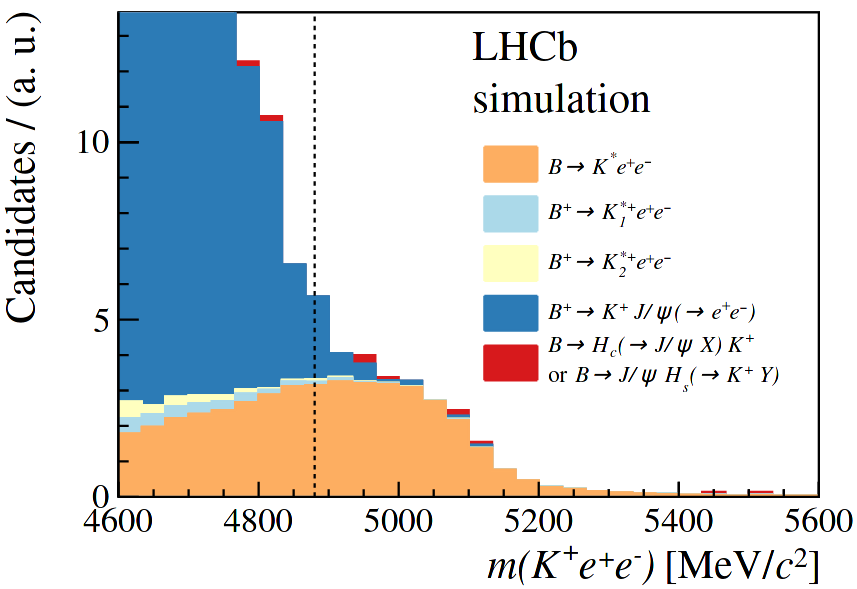
\includegraphics[width=0.8\linewidth]{media/backgrounds.png}
	\caption{Simulated background distributions after applied cuts\cite{petridis2021test}. The dotted line is the lower bound on the selection window.}%
	\label{fig:backgrounds}
\end{figure}

\subsection{Cross-checks}
To verify the experimental procedure 
multiple cross-checks on other variables are performed. 
The efficiencies are tested with 
\begin{equation}
	r_{J/\psi} = \frac{\mathcal{B}(B^+\to K^+J/\psi(\mu^+\mu^-))}{\mathcal{B}(B^+\to K^+J/\psi(e^+e^-))} = 1
\end{equation}
which is a factor in \autoref{eqn:rkexp} and the equality to unity is known within \SI{0.4}{\percent}.
This is not at all trivial, but in fact a very strict test of the procedure, since it requires 
the control of muons relative to electrons.
The measured value is 
\begin{equation}
	r_{J/\psi} = \num{0.981+-0.020}.
\end{equation}
This check is performed for the new and old datasets as well as with different trigger configurations.
Another test is to look at $r_{J/\psi}$ in different kinematic regions, since it should always be compatible with 1.
This is done for two kinematic varibales in \autoref{fig:kinematic}. Since the distribution is 
flat, we are confident that the efficiencies are understood.

\begin{figure}
	\centering
	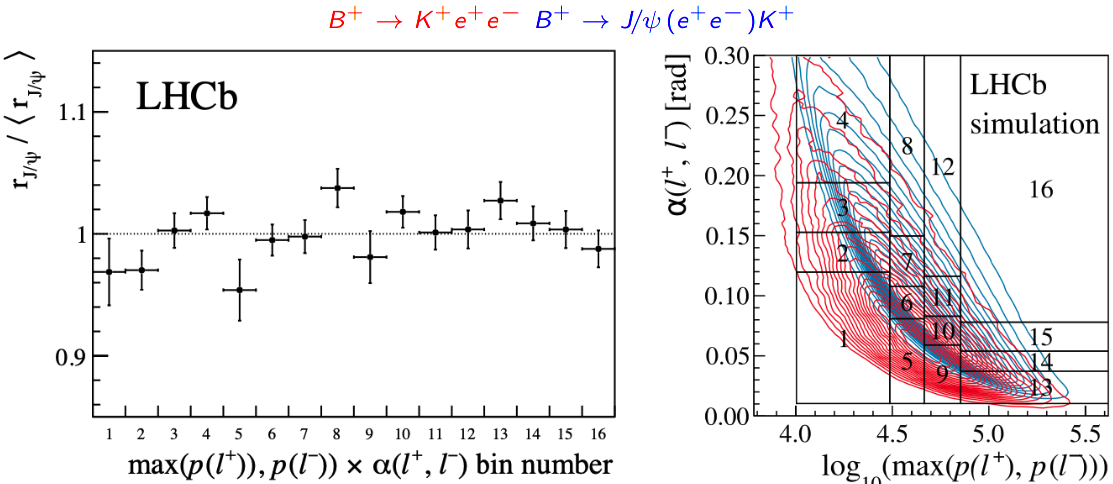
\includegraphics[width=\linewidth]{media/kinematic.png}
	\caption{Cross check of $r_{J/\psi} = 1$ throughout the phase space \cite{petridis2021test}. 
	On the right hand side you can see the binning in the space of the maximal lepton momentum vs the opening angle between the leptons.
	On the left hand side you can see the flat distribution of $r_{J/\psi}$.}%
	\label{fig:kinematic}
\end{figure}

To validate the double-ratio procedure, it is performed on the $B^+\to K^+\psi(2S)(\mu^+\mu^-)$ decay.
The value 
\begin{align}
	R_{\psi(2S)}
	&= \l .\frac{\mathcal{B}(K^+\psi(2S)(\mu^+\mu^-))}{\mathcal{B}(K^+J/\psi(\mu^+\mu^-))} \r/
	\frac{\mathcal{B}(K^+\psi(2S)(e^+e^-))}{\mathcal{B}(K^+J/\psi(e^+e^-))} \nonumber
	\\ &= \num{0.997+-0.011}
\end{align}
is consistent with unity in the $1\sigma$ interval. This can additionally be interpreted 
as the best LFU test in $\psi(2S)\to \ell^+\ell^-$.


\subsection{Systematic uncertainties}
The dominant systematic uncertainties ($\approx \SI{1}{\percent}$) 
are due to the choice of the fit model 
and the statistics of the calibration samples used to understand the backgrounds.
There are smaller systematic sources of uncertainty ($\approx {1}$~\textperthousand)
like the dependency of the definition, the precision of $q^2$ and $m(K^+e^+e^-)$ smearing 
factors.
The total relative systematic uncertainty in the final $R_K$ measurement will be \SI{1.5}{\percent}
and is expected to be dominated by the statistic uncertainties.

\subsection{Measuring $\bfiftextbf{R_K}$}
$R_K$ is now determined as a fit parameter connecting both distributions of 
\autoref{fig:masses}. 
The fit is performed as an extended unbinned maximum likelihood fit.
Extended means that the yields are a fit parameter. 
With this the $R_K$ is measured to be 
\begin{equation}
	R_K = \num{0.846}_{-0.39}^{+0.042}(\text{stat})_{-0.012}^{+0.013}(\text{syst}).
\end{equation}
This gives a $p$-value under SM hypothesis of \num{0.0010}, 
which corresponds to evidence of LFU violation at $3.1\sigma$.
Using previous measurements of $\mathcal{B}(B^+\to K^+\mu^+\mu^-)$
it is possible to calculate $\mathcal{B}(B^+\to K^+e^+e^-)$: 
\begin{equation}
	\frac{\dif \mathcal{B}(B^+\to K^+e^+e^-)}{\dif q^2} = (28.6_{-1.4}^{+1.5}(\text{stat})\pm 1.4(\text{syst}))\cdot 10^{-9} \si{c\tothe{4}\per \giga\electronvolt\tothe{2}}.
\end{equation}
This value implies that electrons seem to behave more SM-like than muons as can be seen in \autoref{fig:lhcbfinal}.
\begin{figure}
	\centering
	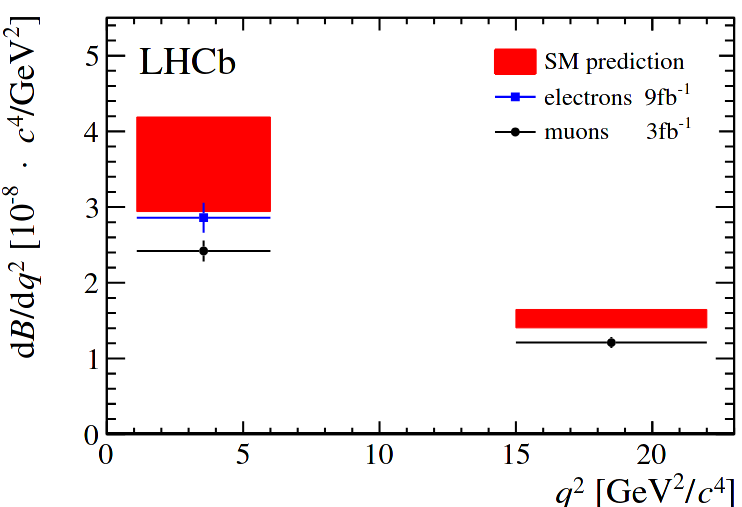
\includegraphics[width=0.8\linewidth]{media/lhcbfinal.png}
	\caption{Differential branching fraction comparing measured results with SM predictions \cite{petridis2021test}.}%
	\label{fig:lhcbfinal}
\end{figure}



\section{Conclusion}
The updated measurement of $R_K$ with the full LHCb dataset 
suggest violation from lepton flavor universality at $3.1\sigma$.
This forms a consistent picture of lepton flavor anomalies,
making future investigations of LFU in these decays very important.
To have a better understanding of this phenomenon more data of 
LHC Run3 is needed.
An independent confirmation of this result by other LHC detectors and 
Belle2 is needed.
